\section{EnergyScope Pathway: The right model to choose} 
\label{app:ESPathway_choice}

Energy system models of varying complexity are valuable tools for guiding policymakers and projecting future trends. These models enable the exploration of different energy scenarios and the assessment of their consequences based on the underlying assumptions. Specifically, techno-economic models play a crucial role in identifying technically feasible pathways for the energy transition while considering the associated economic costs. These models can be classified based on two key factors: technical resolution and simulation horizon, as illustrated in Figure \ref{fig:energy_models_classification}.


\begin{figure}[!htbp]
\centering
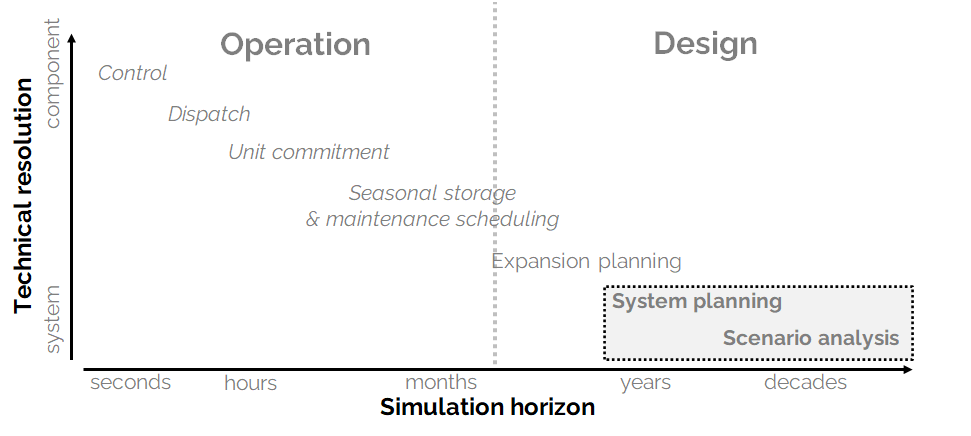
\includegraphics[width=\textwidth]{Models_classification.png}
\caption{Model can be classified by their core focus: \textbf{Operation} or \textbf{Design}. These categories can be broken down into subcategories. This paper focuses on the system planning and scenario analysis models. Inspired from \cite{palmintier2013incorporating}. }
\label{fig:energy_models_classification}
\end{figure}


Increasing the technical resolution of energy system models often comes at the expense of a shorter simulation horizon, and vice versa. For instance, day-ahead grid operation models prioritise accurate grid resolution and capacity reserves for uncertainties, but they may not incorporate long-term market trends. Different model classes cater to various needs, with decreasing technical resolution. These include machine-level control, network dispatch, unit commitment, maintenance, power plant expansion, planning for new infrastructure, and scenario analysis. Each class serves a specific purpose, from fine-grained control within a machine to the exploration of multiple assumptions across different scenarios.

% Specific need & criteria

In accordance with the previous classification, models aimed at aiding decision-makers in the energy transition primarily fall under the categories of planning and scenario analysis, with a relatively lower technical resolution. Nonetheless, ensuring technical accuracy is of paramount importance to ensure the effective functionality of future energy systems. Hence, these models should meet the following requirements as a minimum:
(i) assessment of intermittent renewable energy integration;
(ii) accounting for all energy flows in different sectors, including the measurement of greenhouse gas emissions in the energy sector;
(iii) exploration of all available options;
(iv) consideration of investments throughout the transition process; and
(v) ensuring a reasonable computation time for analysing different trajectories.
Additionally, to enhance result reproducibility and user understanding, it is advantageous for such models to:
(vi) maintain transparency and preferably be open-source, accompanied by collaborative documentation.


These requirements can be transposed into criteria that a model should match:
(i) it should have an hourly resolution spanning a one-year time horizon;
(ii) it should encompass the entire energy system, including all types of demands (such as heat, electricity, mobility, and non-energy
%\footnote{Non-energy demand is often omitted in models while it represents up to 10\%  of worldwide energy demand and up to 20\% in some countries \cite{rixhon2022integration}. \citet{eurostat2019energy} defines the non-energy demand as `\emph{energy products used as raw materials in different sectors, not consumed as a fuel or transformed into another fuel}´.}
), as well as all resources, conversion processes, and storage technologies;
(iii) it should optimise the system design, accounting for all the options;
(iv) it should have a long-term investment horizon, spanning several decades;
(v) its computational time should be reasonable, typically less than one hour on a personal laptop;
(vi) it should be open-source, with accessible data and comprehensive documentation.
These requirements are commonly found in reviews of energy system models. In 2010, \citet{Connolly2010} reviewed 68 tools, considering similar criteria: (i-iv) and (vi), along with others such as the number of users and market equilibrium. In 2019, \citet{prina2019transition} reviewed 12 ``\emph{most established}" models, focusing on criteria (i-ii) and (iv). This review was followed by a classification where criteria (i-iv) were taken into account \cite{prina2020classification}. In 2021, \citet{chang2021trends} conducted a survey-based review of 42 models for energy transition modelling, covering all criteria except computational time.
Based on these reviews, Table \ref{tab:intro_soa} compares models based on all the previous criteria except the computational time (v). Indeed, the latter is hard to compare as models are not apply to the same case study and the information is rarely given. The table includes only the models that achieved partially at least four out of the five criteria. The authors endeavored to refresh the model's information by consulting the model's website and repository, yet there is a possibility that some information might have been overlooked or omitted inadvertently.

\begin{table}[!htbp]
\caption{Comparison of existing models that partially satisfy at least four of the six criteria (in alphabetical order). Legend: \checkmark criterion satisfied; {\color{gray} \checkmark} criterion partially satisfied; {\color{gray} \xmark} criterion not satisfied. Data from \cite{Connolly2010,prina2020classification,chang2021trends,prina2019transition}.}
\label{tab:intro_soa}
\begin{minipage}{\textwidth}
\centering
\resizebox{\textwidth}{!}{
\begin{tabular}{lcccccc}
\toprule
\textbf{Model} & \textbf{Ref.} & \textbf{Hourly} & \textbf{\parbox{2cm}{\centering Whole-energy}}& \textbf{\parbox{2cm}{\centering Optimis. invest. \& operation}} & \textbf{Pathway} & \textbf{\parbox{2cm}{\centering Open-source}} \\
\midrule
Calliope & \cite{Atlason2014,Calliope} & \checkmark & \checkmark & \checkmark & {\color{gray} \xmark}\footnote{Topic is being discussed in the chat of their repository but not yet included in their documentation.} & \checkmark \\
COMPOSE & \cite{COMPOSE} & \checkmark & \checkmark & \checkmark & \checkmark & {\color{gray} \checkmark}\footnote{\label{foot:freeundersomespecial}`\emph{Free under some special conditions}´.} \\
DER-CAM & \cite{popovic2017mixed,dercam_website} & \checkmark & {\color{gray} \checkmark}\footnote{\label{foot:transportnotsaid} Transport not accounted.}\footnote{\label{foot:industrynotaccounted} Industry not accounted} & \checkmark & {\color{gray} \xmark} \footnote{\label{foot:notpathway} Not specified but time horizon is 1 year.} & {\color{gray} \checkmark} \footnote{\label{foot:freeware} Freeware.} \\
DIETER & \cite{zerrahn2017long} & \checkmark & {\color{gray} \checkmark} \footref{foot:industrynotaccounted}\footnote{\label{foot:dhnnotaccounted} \gls{DHN} not accounted.} & \checkmark & {\color{gray} \xmark}\footref{foot:notpathway} & \checkmark \\
E2M2 & \cite{E2M2} & \checkmark & {\color{gray} \checkmark} \footref{foot:transportnotsaid}\footref{foot:industrynotaccounted}\footnote{\label{foot:decLTHnotaccounted} individual heating not accounted.} & \checkmark & \checkmark & {\color{gray} \xmark}\footnote{\label{foot:paidlicenced} Commercially (paid) licensed.} \\
EMPIRE & \cite{backe2022empire} & \checkmark & {\color{gray} \xmark} \footref{foot:transportnotsaid}\footref{foot:industrynotaccounted}\footref{foot:dhnnotaccounted}\footref{foot:decLTHnotaccounted} & \checkmark & \checkmark & {\color{gray} \checkmark}\footref{foot:freeundersomespecial} \\
Ener. Trans. Model & \cite{ETM} & \checkmark & \checkmark & {\color{gray} \xmark} \footnote{The ETM is a simulation model with a simple merit order 'optimisation' for electricity, flex and heat.} & \checkmark & \checkmark \\
EnergyPLAN & \cite{lundenergyplan} & \checkmark & \checkmark & {\color{gray} \xmark} \footnote{\label{foot:simulation} Simulation model.} & {\color{gray} \xmark} \footnote{\label{foot:notpathwaystated} Yearly horizon without pathway.} & {\color{gray} \checkmark}\footref{foot:freeware} \\
energyRt & \cite{EnergyRT} & \checkmark & \checkmark & {\color{gray} \checkmark} \footnote{\label{foot:invopt} EnergyRT optimises investments only, while iHOGA conducts optimisation and simulation without specifying timing or scope.} & \checkmark & \checkmark \\
EnergyScope TD & \cite{limpens2019energyscope} & \checkmark & \checkmark & \checkmark & {\color{gray} \xmark} \footref{foot:notpathwaystated} & \checkmark \\
Enertile & \cite{enertile} & \checkmark & \checkmark \footref{foot:industrynotaccounted} & \checkmark & \checkmark & {\color{gray} \xmark} \footnote{ Only for internal use.} \\
ESO-XEL & \cite{heuberger2017electricity} & \checkmark & {\color{gray} \xmark}\footref{foot:transportnotsaid}\footref{foot:industrynotaccounted}\footref{foot:dhnnotaccounted}\footref{foot:decLTHnotaccounted} & \checkmark & \checkmark & \checkmark \\
GENeSYS-MOD & \cite{loffler2017designing} & \checkmark & \checkmark & \checkmark &  \checkmark\footnote{\citet{loffler2017designing} applied a pathway transition, but the time resolution was increased to 12h and it uses 3 typical days over a year. \cite{bartholdsen2019pathways} performed a multi-regional pathway (16 nodes) for the case of Germany from 2020 to 2050 with a time step of 5 years. However, the time resolution is 16 time slices representing 4 hours per day and one day per season.} & \checkmark \\
H2RES & \cite{herc2021energy} & \checkmark & {\color{gray} \xmark}\footnote{\label{foot:h2res} In their review in 2021, \cite{prina2021bottom} classified H2RES as a simulation model on power sector only. In their work \cite{herc2021energy} presented a new version of H2RES claiming to optimise the power system and partially represent other sectors. Their study applied the model to a transition pathway for Croatia. In the conclusion, it is claimed `\textit{H2RES offers practically unlimited potential for functionality expansion since it is an open-source program}´ which open the doors for future developments to encompass new features.} &  {\color{gray} \checkmark}\footref{foot:h2res} & \checkmark & \checkmark \\ 
iHOGA & \cite{ihoga} & \checkmark & {\color{gray} \xmark}\footref{foot:transportnotsaid}\footref{foot:industrynotaccounted}\footref{foot:dhnnotaccounted}\footref{foot:decLTHnotaccounted} & {\color{gray} \checkmark} \footref{foot:invopt} & \checkmark & {\color{gray} \checkmark} \footref{foot:freeundersomespecial} \\
IMAKUS & \cite{kuhn2012iteratives} & \checkmark & {\color{gray} \checkmark}\footref{foot:transportnotsaid}\footref{foot:industrynotaccounted} & \checkmark & \checkmark & {\color{gray} \xmark} \footref{foot:paidlicenced} \\
OpenDSS & \cite{opendss} & \checkmark & \checkmark & {\color{gray} \xmark} \footref{foot:simulation} & \checkmark & \checkmark \\
Plexos & \cite{energyexemplarplexos9} & \checkmark & {\color{gray} \checkmark}\footnote{Does not account for all sectors but allow to implement them according to \cite{waucquez2023validation}.} & \checkmark & \checkmark & {\color{gray} \xmark}\footref{foot:paidlicenced}  \\
PyPSA & \cite{brown2017pypsa,PyPsa} & \checkmark & \checkmark & \checkmark & {\color{gray} \checkmark} \footnote{\cite{pedersen2022long} applied PyPSA to a whole energy system split in 37 nodes. Using a myopic approach, the model optimises the energy transition with a 3-hours resolution). } & \checkmark \\
RamsesR & \cite{energistyrelsen2023ramses} & \checkmark & {\color{gray} \checkmark}\footref{foot:transportnotsaid}\footref{foot:industrynotaccounted}\footref{foot:decLTHnotaccounted} & \checkmark  & \checkmark & \checkmark \\
ReEDS & \cite{short2011regional} & {\color{gray} \xmark}\footnote{ Seasonal time slice.} & {\color{gray} \checkmark}\footref{foot:industrynotaccounted}\footref{foot:dhnnotaccounted}\footref{foot:decLTHnotaccounted} & \checkmark & \checkmark & {\color{gray} \checkmark} \footref{foot:freeundersomespecial} \\
TIMES & \cite{loulou2005documentation} & \checkmark & \checkmark & \checkmark & \checkmark & \checkmark\footnote{Model is now open-source with limited access to data \cite{openmod_times_description}.} \\
\bottomrule
\end{tabular}}
\end{minipage}
\end{table}


From Table \ref{tab:intro_soa}, four models almost check all the boxes (partially the pathway one): Calliope, GENeSYS-MOD, PyPSA and TIMES. 
The TIMES model, short for The Integrated MARKAL-EFOM System, is a well-established framework renowned for its capacity to generate comprehensive energy models. It encompasses a rich array of features, including support for multi-cell modeling, pathway analysis, full-scale representation of energy systems, and the consideration of market equilibrium dynamics, all of which facilitate thorough scenario exploration. This model has a widespread adoption and has been utilized by worldwide institutions such as the \gls{IEA} or technical ones such as VITO (Vlaamse Instelling voor Technologisch Onderzoek) research institute in their research endeavors. Notably, TIMES was reported commercial in 2010 \cite{Connolly2010}. A more recent survey conducted in 2020-2021 confirmed that the model was using a commercial interface \cite{chang2021trends}. Recent developments by the IEA-ETSAP have resulted in a version that is compatible with open-source solver CBC. In various studies conducted in different regions, including Canada, Sweden, the EU, and Denmark, TIMES has been shown to utilize 12 to 32 time-slices annually \cite{prina2020classification}. It is noteworthy that \citet{haydt2011relevance} conducted a study focusing on the electrical sector, using 288 time slices, equivalent to a 12-day time resolution, highlighting the sensitivity of results to time resolution. Regarding data accessibility, while some publications partially present the dataset used, the overall accessibility of TIMES data remains an area of ongoing inquiry \cite{openmod_times_description}. 
 Calliope is a `\emph{tool that makes it easy to build energy system models}´ at different geographical scale. Even if the framework offers the possibility of modelling multi-year systems, the authors didn't find a relevant publication on this topic. In fact, the model is typically employed for scenario analysis with a specific focus on the electricity system. Previous studies have used the model to investigate the phasing out of fossil and nuclear energies in a multi-regional UK power system \cite{pfenninger2015renewables}. More recently, the model has been applied to analyse a scenario of a multi-energy district in Switzerland \cite{pickering2021quantifying}. Moreover, the model has been used with decades of weather data. However, its application has been limited to assessing the impact of inter-year variability in wind and PV on the results, rather than evaluating a transition pathway \cite{pfenninger2017dealing}. 
Similarly GENeSYS-MOD presents some limitations. This model is an application of the open-source energy modelling system (OSeMOSYS), itself represented as a model with a poor time discretisation and a heavy computational burden according to 
\cite{prina2019transition}. \citet{loffler2017designing} applied the model to the world by splitting it into 10 regions and most of the energy demand sectors. The time disaggregation can be chosen by the user, for their application they used representative years with three days and two time slice per day. 
%\cite{bartholdsen2019pathways} performed a similar study for the case of Germany with 16 time slices per representative years and motivated this choice as sufficient as \cite{welsch2014incorporating} demonstrates that it gives consistent results compared to using hourly time resolution over a year.  However, with limited number of time slices, storage technologies, especially the ones for inter-month storage, cannot be optimised and thus simplifies the non-yet solved challenge of intermittent renewable energy integration. 
%PyPSA, one of the most promising model thanks to its strong and active community, has also been used to perform a myopic transition \cite{pedersen2022long}.  
Among the open-source models with an active community, PyPSA is one of the best-performing, with a large and active community, development at the state of the art, worldwide applications, and usage not only limited to academia. A study conducted by \citet{bartholdsen2019pathways} centered on Germany employed a representation comprising 16 time slices for representative years. This choice was substantiated by the work of \citet{welsch2014incorporating}, which demonstrated that this level of temporal granularity yields consistent results in comparison to hourly time resolution over a year. However, it is noteworthy that the utilization of a limited number of time slices may simplify the optimization of storage technologies, especially those designed for inter-month energy storage. This simplification can be viewed as a pragmatic approach to reduce the computational burden while over-simplifying the challenge of accurately integrating intermittent renewable energy sources. Furthermore, PyPSA, a modeling framework recognized for its robustness and active user community, has also been employed to investigate scenarios related to myopic transitions \cite{pedersen2022long}. 
Hence, it is worth noting that while Calliope, OSeMOSYS, PyPSA and TIMES frameworks have the potential to be used for evaluating a transition pathway, the authors have not come across any publication that explicitly demonstrates their application to such cases with an hourly time resolution over significant time slices. 



% SOA

Hence, it appears that none of the models of Table \ref{tab:intro_soa} fully meet all five criteria outlined in the table, topped with the additional consideration of acceptable computational time. This observation is consistent with the findings presented in \cite{prina2019transition} who identified two approaches for optimising the energy transition pathway based on the six criteria. The first approach involves running a snapshot model multiple times using an algorithm that optimises the transition path and validates the system's operability. The second approach aims to extend a snapshot model to represent the entire transition pathway. However, they excluded this option due to the lack of models that met the requirements of being fast enough and easily adaptable. 
Therefore, they developed a new model based on the first methodology, named EPLANoptTP. It uses a multi-objective evolutionary algorithm to optimise the EnergyPLAN model \cite{lundenergyplan}. To manage computational time, the number of decision variables is limited to three: \gls{PV}, wind turbine and battery capacities. Thus, the model does not investigate all the options (\ie criteria (iii)). 



